In addition to the regular spin-down of radio pulsars due to magnetic braking,
some pulsars undergo anomalies in their timing solutions known as
\emph{glitches}.  These are sudden rapid increases in the pulsation frequency
which were first observed in the Crab \citep{Boynton1969, Richards1969} and
Vela pulsars \citep{RadhakrishnanManchester1969, Reichley1969}. Pulsar
timing methods model this as a permanent increase in the phase, frequency, and
first frequency derivative in addition to a frequency increment that
subsequently decays exponentially to zero \citep{Edwards2006}.  To model this,
for each glitch pulsar astronomers add on an additional term to
Eqn.~\eqref{eqn: Taylor compact}:
\begin{align}
\begin{split}
\phi_{\textrm{g}} = H(t - \tg)& {}\left(
\Delta\phi + \Delta\nu(t - \tg) + \frac{\Delta\dot{\nu}}{2}(t - \tg)^{2} \right.\\
& \hspace{3mm}+ \left.\left[1-\exp\left(-\frac{t - \tg}{\tau}\right)\right]
\Delta\nu_{\textrm{t}}(t - \tg)
\right),
\end{split}
\label{eqn: glitch timing model}
\end{align}
where $H(t)$ is the Heaviside step function. The first
three terms are the permanent increase in phase, frequency, and spin-down,
while the last term gives the transient increase in the frequency
$\Delta\nu_{\textrm{t}}$ which decays exponentially with a timescale $\tau$.
To illustrate this, in Figure~\ref{fig: glitch sketch} we show the spin-frequency
model of a glitch including a permanent increase in frequency $\Delta\nu$ and
a component $\Delta\nu_{\textrm{t}}$ which is `recovered'.
\begin{figure}[htb]
\centering
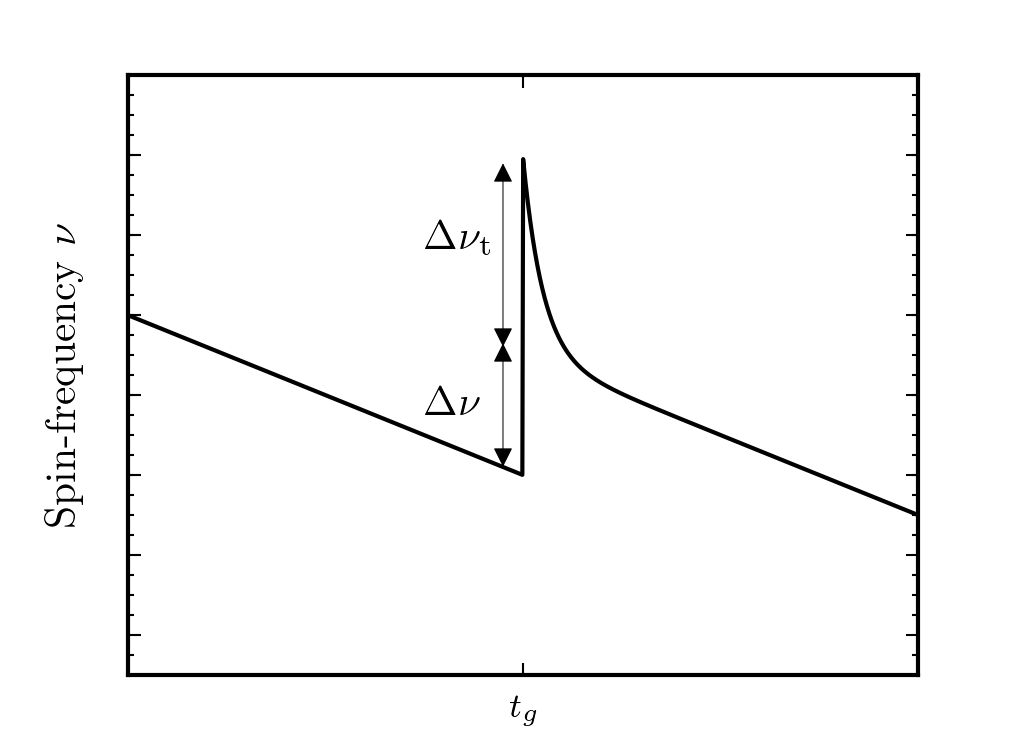
\includegraphics[]{glitch_sketch}
\caption{Illustration of the glitch model fitted by pulsar astronomers.}
\label{fig: glitch sketch}
\end{figure}

In effect, pulsar astronomers fit separate Taylor expansions either side of the
glitch. This is a good model when the rise-time of the glitch, during which the
frequency increases, is short compared to the duration between observations.
This evolution of the frequency during a glitch has yet to be observed, but
high time resolution monitoring of the Vela pulsar placed an upper limit of
40~s for the rise-time between the original and the new period
\citep{Dodson2001}. Since we cannot resolve the glitch itself,
Eqn.~\eqref{eqn: glitch timing model} is appropriate and used for all known
glitches.

A comprehensive review of glitches was carried out by
\citet{Espinoza2011}; to illustrate a typical glitch, in Figure~\ref{fig: glitch}
we reproduce data from this review on a glitch in the Crab pulsar.
\begin{figure}[htb]
    \centering
    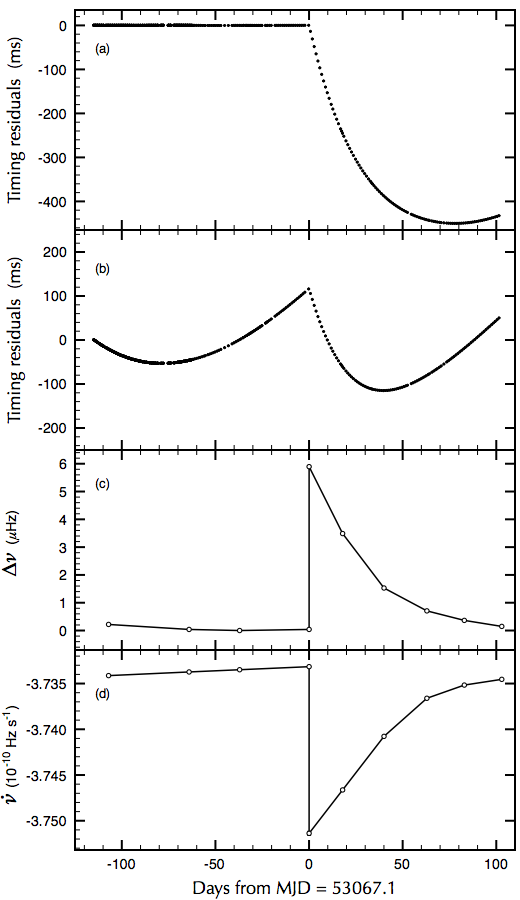
\includegraphics[width=0.5\textwidth]{GlitchExample_jbman}
    \caption{
A glitch in the PSR B0531+21, the Crab pulsar. It occurred around MJD
53067 and had a fractional frequency jump of $\Delta\nu/\nu = 5.33 \pm 0.05
{\times}10^{−9}$. (a) The timing residuals relative to a
slowdown model with two frequency derivatives when fitting data only up to the
glitch date. (b) Timing residuals after fitting all data in the plot; note
that the glitch feature is still visible. Both these panels have the same
scale, covering 500 ms. (c) Frequency residuals, obtained by subtracting the
main slope given by an average $\dot\nu$. (d) The behaviour of $\dot\nu$
through the glitch. This figure and caption are adapted from Figure~(1) of
\citet{Espinoza2011}.}
    \label{fig: glitch}
\end{figure}

Over 165 of the $\sim$2000 observed pulsars have been seen to glitch, often multiple
times. Typical values of the instantaneous frequency change range from
$10^{-9}$~Hz to $10^{-4}$~Hz For some pulsars this is accompanied by a change,
with either sign, in the spin-down rate $\Delta\dot{\nu}$ with absolute
magnitudes between $10^{-19}$~Hz/s to $10^{-12}$~Hz/s.
In most pulsars the \emph{glitch recovery parameter}, defined as
\begin{align}
Q = \frac{\Delta\nu_\textrm{t}}{\Delta\nu + \Delta\nu_\textrm{t}},
\end{align}
can not be measured. This may be due either to infrequent observations of the
pulsar, or simply that $Q\ll1$.  A review of pulsars with measured values of
$Q$ was conducted by \citet{Lyne2000}; they found that in glitches from 18
pulsars, $Q$ correlates with $|\dot{\nu}|$ reaching values as large as
$\sim0.9$ for the youngest pulsar with the highest absolute spin-down rate,
the Crab pulsar.

Many pulsars have been observed to glitch several times, \citet{Melatos2008}
considered the waiting times between glitches and concluded that in most
glitching pulsars the glitches happen randomly with waiting times consistent
with a Poisson process, except in PSR J0537-6910 and PSR J0835-4510 which
displayed quasi-periodicity in the waiting times.

In Chapter~\ref{sec: glitches in cgw}, we perform our own investigation into the
population statistics of glitches with an aim to understand their implication
for gravitational wave searches. We find, in agreement with
\citet{Espinoza2011} and references therein, that the distribution of glitch
magnitudes has multiple modes which suggests that glitches may come from more
than one mechanism. We go on to apply a statistical model and determine empirically
the properties of the underlying source populations.

Glitches provide a unique opportunity to investigate the physics of neutron
stars and many of the leading insights have been gained by their study. Two
leading models exist known as the \emph{superfluid unpinning} model and the
\emph{starquake} model.

In the superfluid unpinning model proposed by \citet{Anderson1975}, the star
contains a superfluid component in which the angular momentum is stored in an
array of vortices which are `pinned' to the crust. The magnetic dipole, rigidly
fixed to the crust, exerts a torque on the crust gradually spinning it down.
The superfluid component cannot decrease its angular momentum without reducing
the number of vortices per unit area, so does not spin down at the same rate. A
lag in frequency between the superfluid component and rest of the crust
develops until the forces are sufficiently large to cause an avalanche of
unpinning events rapidly transferring the stored angular momentum in the
superfluid component to the crust. An observer measures the frequency and
spin-down rate from the rate of pulsations. These pulsations originate from the
EM dipole which is frozen into the crust of the star, so when this unpinning
occurs, we see a rapid increase in the frequency.

The second model, starquakes, follows from the observation that a rapidly
spinning fluid body has an oblate `rest shape' with a bulge about its equator
due to the centrifugal force. The crust of a star spinning at a some frequency
will solidify with a corresponding oblateness which we call the reference
oblateness. Subsequently, as the star spins down, it will have a different rest
oblateness due to its decreased frequency, but the crust will retain a memory
of the earlier reference oblateness at which it solidified. This will cause
strains in the crust which eventually cause a starquake relieving the strain,
resetting the reference rest shape, and producing glitch like features. This
model was first proposed by \citet{Ruderman1969} and later built upon by
\citet{Baym1971}.

Both of these models have support in the literature and have been developed
significantly to explain the variety of observed glitches. However, there are
observations which cause difficulties for both models: glitches seen in the
Vela pulsar are too large and too often to be consistent with a starquakes
model, while the unpinning model requires a superfluid component which is at
odds with observation of precession (we discuss this further in
Chapter~\ref{sec: testing models}). In this thesis, we will not use glitches
as a tool for inferring neutron star physics, but any predictions we do make
must be compatible with what has already been learnt from glitches.


